
\documentclass[12pt,english]{article}
\usepackage[utf8]{inputenc}
\usepackage{tgpagella} %
\usepackage{mathpazo}  %
\usepackage[left=1.5in,right=1.5in,top=1.5in,bottom=1.5in]{geometry}
\usepackage[natbibapa]{apacite}
\bibliographystyle{apacite} 
\usepackage{url} %
\usepackage[hyperpageref]{backref} %
\usepackage[pagebackref]{hyperref} %
\hypersetup{
  colorlinks=true, %
  urlcolor=purple,    %
  linkcolor=blue,  %
  citecolor=violet,   %
}
\usepackage{bm}
\usepackage{indentfirst}
\setcitestyle{aysep={}} 
\usepackage{amsmath}
\usepackage{tcolorbox}
\usepackage{amssymb}
\usepackage{eurosym}
\usepackage{amsfonts}
\usepackage{enumerate}
\usepackage{babel}
\usepackage{graphicx}
\usepackage{caption}
\usepackage{supertabular}
\usepackage{tabularx}
\usepackage{float}
\usepackage{dsfont}
\usepackage{fancyvrb}
\usepackage{verbatim}
\usepackage{enumitem}
\usepackage{setspace}
\usepackage{comment}
\usepackage{subcaption}
\usepackage{tikz}
\usepackage{gensymb}
\usepackage{textcomp}
\usepackage{placeins} %

\usepackage{tabulary}
\usepackage{tabularx}
\usepackage{booktabs}
\usepackage{fullpage}
\usepackage{morefloats}
\usepackage{makecell}
\usepackage{lscape}
\usepackage{pdflscape}
\usepackage{longtable}
\usepackage{rotating}
\usepackage{fancyhdr}
\usepackage{tocbibind} %
\usepackage{titletoc} %
\usepackage[export]{adjustbox}
\usepackage[anythingbreaks]{breakurl} %
\usepackage{multicol}
\usepackage{lineno}
\usepackage{endnotes}
\let\footnote=\endnote
\makeatletter
\renewcommand\tableofcontents{%
    \@starttoc{toc}%
}
\makeatother
\newsavebox\ltmcbox %
\renewcommand{\floatpagefraction}{.99}
\newenvironment{stretchpars}{\par\setlength{\parfillskip}{0pt}}{\par} %
\title{Shortfall of Domestic Resources\\ to Eradicate Extreme Poverty by 2030} 
\date{\today} %

\begin{document}

\sloppy
\maketitle
\begin{abstract}
In 2015, the Sustainable Development Goals set the eradication of extreme poverty by 2030 as a universally agreed objective. This paper analyses the prospects for achieving this goal country by country. Without a reduction in inequality, even with a very optimistic annual growth rate of 7\% between 2022 and 2030, 3\% of humans would still be living in extreme poverty in 2030. National capacity to eradicate poverty is then measured using the concepts of \textit{antipoverty cap} or \textit{antipoverty tax} required to finance poverty eradication, and \textit{income floor} (financed by a given income tax). With credible annual growth of 3\%, even capping incomes at \$7 a day (to finance an increase in incomes for the poorest individuals) cannot eradicate extreme poverty in 5 low-income countries. In other words, neither growth alone nor growth combined with radical domestic redistribution could eradicate extreme poverty by 2030. By contrast, a transfer of just 0.15\% of global income could achieve this goal. This could be financed by a 2\% tax on individual net wealth above \$1 billion.

\end{abstract}
\clearpage
\tableofcontents

\section{Introduction}%

The very first Sustainable Development Goal (SDG) %
reads: ``By 2030, eradicate extreme poverty for all people everywhere, currently measured as people living on less than \$2.15 a day''. As we have passed the halfway point since the adoption of the SDGs in 2015, it is time to assess progress towards this universally accepted goal. 

In this paper, I assess whether growth and domestic redistribution are sufficient to eradicate extreme poverty by 2030. I first study the extent of poverty in different growth scenarios. Then, I calculate the magnitude of domestic redistribution required in each country to eradicate poverty in 2030. I mobilize different indicators. For two idealized tax policies, I estimate the parameter that would raise enough revenue to eradicate poverty. In the ``antipoverty cap'', I fix the tax rate at its maximum value of 100\% so that the tax effectively becomes a cap on top incomes, and I find the required cap (or taxation threshold). All income above the cap is assumed to be redistributed to the lowest incomes in order to eradicate poverty. In the ``antipoverty tax'', I fix the taxation threshold and find the tax rate needed to raise the revenue required to eradicate poverty. As a last indicator, the ``income floor'', I fix both the taxation threshold and the tax rate, and I compute the income floor that the tax could finance (by redistributing tax revenue to the lowest incomes). In the lowest income countries, extreme poverty is estimated to persist even after strong growth and radical redistribution. %
This has implications for the international community, as international solidarity appears necessary to achieve the first SDG. I complete the analysis by exemplifying international transfers that would eradicate poverty by 2030.

To assess the prospects of achieving the first SDG, I explore in turn the effects of balanced growth alone, idealized national redistribution policies, and idealized global redistribution. The thought experiments are not meant to be exhaustive or representative pathways to achieving the first SDG. They are presented to demonstrate that relying on growth and domestic policies alone would fall short of eradicating poverty by 2030. This impossibility result is robust to a wide range of growth and redistribution scenarios, including extremely optimistic ones. In contrast, global solidarity has the potential to dramatically accelerate poverty eradication.

\paragraph{Literature} 

The idea to measure the domestic capacity to eradicate poverty with an antipoverty cap originates in \cite{medeiros_rich_2006} (who calls it the ``affluence line''). In turn, the idea to measure it with an antipoverty tax dates back to \cite{ravallion_poorer_2010} and \cite{ceriani_income_2014} (the latter dub it ``income lever''). \cite{ravallion_poorer_2010} found that even with a 100\% tax above the U.S. poverty line, 29 countries could not eradicate extreme poverty, and 37 countries could not eradicate ``severe poverty'' defined with a higher poverty line (which corresponds to \$3.65/day in 2017 PPP \$). %
\cite{bolch_arithmetics_2022} --- hereafter ``BCL'' --- update the computations with more recent data and find that 62 countries do not have sufficient resources to eradicate severe poverty. %

The present paper employs a similar methodology to assess which countries have sufficient domestic resources to achieve the first SDG. There are three reasons why BCL cannot be used %
for that purpose. 
First, the most recent data was not available to BCL (their most recent survey year is 2012 with most years in 2009--2010, compared to 2018--2021 in the present paper). %
Second, BCL study the data as it stands rather than adjusting it for growth and using it to infer the income distributions in 2030. Third, they focus on a poverty line higher than the one officially used in the first SDG.

In contrast to BCL, I find that 34 countries lack sufficient resources eradicate severe poverty in 2030 in a scenario with 3\% growth. Compared to BCL, this less pessimistic finding is largely due to growth up to 2030; though the revision of inequality data also plays a role (see Section \ref{subsec:cap}). 

Consistently with \cite{ravallion_poorer_2010}, \cite{hoy_gasoline_2016} find that 52\% of global extreme poverty can be eliminated with a 50\% antipoverty tax above \$$_\text{2011}$10/day (in 2011 PPP). They also consider the reallocation of public spending and show that this antipoverty tax together with the reallocation of fossil-fuel subsidies and military spending could eliminate 77\% of global extreme poverty. Finally, they show that countries with GDP per capita below \$$_\text{2011}$2,000 per year do not have the domestic capacity to eradicate extreme poverty (measured as an antipoverty tax below 50\%).

\cite{woodward_incrementum_2015} also shows that with growth alone, and if each country's growth persists at the same level, it would take more than a century --- and a global GDP p.c. exceeding \$100,000 per year --- to end extreme poverty. %
\cite{ortiz_universal_2018} find that financing a basic income at the poverty line is out of reach in low-income countries as the national poverty line is on average equal to 79\% of the GDP p.c. and 8 countries have a GDP p.c. below this line (which is often itself below \$2.15/day).

The paper also relates to estimates of future poverty rates based on growth alone. Using GDP projections from the IMF, \cite{karver_mdgs_2012} project the 2030 extreme poverty rate at 2.8\% (and at 4.1\% if growth is 1\% lower than projected, the error historically observed with IMF projections). Other studies are more pessimistic, at 3--7\% \citep{chandy_final_2013,bicaba_can_2017}, 4.7\% \citep{manuel_financing_2018} or even 7.4\% for post-COVID estimates \citep{lakner_how_2022}. 

The paper is linked to the literature that estimates the global income distribution \citep{pinkovskiy_parametric_2009,anand_chapter_2015,lahoti_global_2016,lakner_global_2016,gradin_trends_2021,jorda_global_2019,alvaredo_methods_2021,fisher-post_government_2023,milanovic_three_2024}. 
I follow \cite{lakner_global_2016} by merging income and consumption data without adjustment in the main specification. 
\cite{anand_chapter_2015} discuss common issues regarding the global income distribution and introduce a method to handle discrepancies between data sources. I follow a similar method as a robustness check, as explained in Section \ref{subsec:data}. 

The paper also connects with the costing and progress assessment of SDGs and in particular poverty eradication \citep{schmidt-traub_investment_2015,rozenberg_beyond_2019,sdsn_sdg_2019,manuel_financing_2020,vorisek_understanding_2020,unctad_estimating_2021,un_sustainable_2022}. In 24 countries, a growth rate of 7\% would not suffice to eradicate extreme poverty by 2030 \citep{unctad_estimating_2021}. While the global cost of achieving the SDGs may be as high as \$4 trillion per year \citep{unctad_world_2023}, %
the financing gap in low- and lower-middle-income countries is estimated at \$400 billion \citep{sdsn_sdg_2019} %
to \$700 billion per year \citep{kharas_building_2019}. %
With the current trend, the SDGs will not be achieved and only limited progress towards them will have been made, with more than 60 countries failing to eradicate extreme poverty by 2030 \citep{moyer_are_2020}. %
\cite{manuel_financing_2018} find that low-income countries do not have the resources to afford basic healthcare, education, and social protection; only an increase and a redirection of Official Development Assistance (ODA) can finance these programs. 

The main contribution of this paper is to provide an explicit assessment of the prospects for achieving the first SDG under ideal circumstances. While existing studies estimate the poverty reduction that can be achieved through either growth or domestic redistribution, I study the combination of both. I also introduce the notion of \textit{income floor} as a measure of the credible potential for redistribution. Finally, I improve upon existing studies by presenting results in the form of world maps and by providing an open source code to work with global inequality data: [\textit{removed for the review process}]. This code offers ready-to-use functions to compute all sorts of inequality indicators (Gini, top 10\% share, antipoverty tax rate, etc.) and plot world maps of these indicators.

The rest of the paper is structured as followed: Section \ref{subsec:data} describes the data used in the analysis. Section \ref{sec:results} presents the results: Section \ref{subsec:balanced_growth} assesses the effects of growth on poverty; Section \ref{subsec:method} presents the method to measure domestic capacity to eradicate poverty; Sections \ref{subsec:cap}, \ref{subsec:tax}, and \ref{subsec:floor} analyze respectively the antipoverty cap, the antipoverty tax, and the income floor; Section \ref{subsec:global} indicates how global redistribution could eradicate poverty. Section \ref{sec:conclusion} concludes.

\section{Data}\label{subsec:data}
The percentiles of each country's post-tax income (or consumption) are estimated by the Poverty and Inequality Platform (PIP) of the World Bank (ex-PovcalNet). PIP aggregates the most recent household surveys (59\% of the 167 countries were surveyed between 2018 and 2021). This data is based on purchasing power parity (PPP) and given in constant 2017 \$. PIP data is %
at the individual level, assuming an equal split of income (or consumption) among all household members, including children. %

In low-income countries (those of greatest interest to us), PIP provides data on per capita \textit{consumption} (rather than income). Thereby, the data does not capture services procured by the government. 
Another potential concern with household surveys is that the aggregate (national) consumption they imply is generally lower than the one estimated in national accounts \citep{deaton_measuring_2005,prydz_disparities_2022,hlasny_impact_2022}. This discrepancy comes from measurement errors on both sides: on the one hand, household surveys suffer from underreporting of top incomes and large expenditures; on the other hand, national accounts do not properly account for informal work %
and tend to inflate agricultural output \citep{angrist_why_2021}. 
Furthermore, authoritarian countries have been shown to produce inflated GDP statistics, except for countries below the GDP threshold of eligibility for preferential loans by the World Bank \citep{martinez_how_2022}. %
While Household Final Consumption Expenditures (HFCE) from national accounts is 42\% greater than the aggregate consumption from household surveys, the ``discrepancy ratio'' is largest for middle-income countries and is only 11\% for low-income countries. 
Because household surveys are best suited to estimate consumption by the poorest, I use unadjusted PIP data as a baseline. 

As a robustness check, I also re-derive the main results after adjusting aggregate consumption by the discrepancy ratio (computed using World Bank data). In line with \cite{lakner_global_2013} and \cite{anand_chapter_2015}, I impute the extra consumption to the top percentile. I do not perform the rescaling on the 15\% of countries (like Burundi or the D.R.C.) with HFCE lower than its aggregate consumption from PIP, and I assume a discrepancy ratio of +11\% for the 20\% of countries lacking data on HFCE. 

As is common in this literature \citep{karver_mdgs_2012,hellebrandt_future_2015,bicaba_can_2017}, my baseline assumes ``balanced growth'', meaning that each percentile grows at the same rate between the country's survey year and 2030. This assumption allows separating the effects of growth alone from those of a change in the income distribution. 
I rescale incomes by the observed growth of GDP p.c. (in PPP) up to 2022 (using World Bank data) and by different methods for the 2022--2030 period. 
These methods include: extending the 2014--2019 country growth trend (which excludes COVID years); extending the trend for growing countries and assuming no growth when GDP p.c. has contracted between 2014 and 2019; assuming a constant growth (of either 0\%, 3\%, 4.5\%, 6\%, or 7\%); using IMF forecasts (\cite{imf_world_2023} extended up to 2030 by replicating the 2026--2028 forecasted growth in 2028--2030); projecting future growth using an autoregressive quadratic model that predicts the 2011--2019 growth based on the 1991-2011 growth (then applied to 2022--2030 using the 2002--2022 growth). Besides, I deviate from this two-step procedure to assess the original SDGs, 
by assuming a constant growth of 7\% starting in 2015. In Supplementary Material, I also analyze a path of unbalanced growth that extends recent trends in national inequality to 2030.  

\section{Results\label{sec:results}}
\subsection{The effect of balanced growth\label{subsec:balanced_growth}}

To estimate global poverty rates, the World Bank scales up the percentiles measured in household surveys by the country's GDP growth between the survey year and the year of interest.\footnote{The World Bank also adjusts growth rates when data captures consumption rather than income, cf. \href{https://datanalytics.worldbank.org/PIP-Methodology/lineupestimates.html\#extrapolations}{datanalytics.worldbank.org/PIP-Methodology/lineupestimates.html}.} I project global poverty rates and poverty gaps in 2030 using the same assumption of balanced growth (i.e., constant inequality), for a range of growth scenarios (Table \ref{tab:poverty}). I also show that the balanced growth assumption has little effect on poverty estimates compared to an alternative assumption of unbalanced growth in which national inequality evolves as in the recent past (see Supplementary Material for details). This is because inequality has been quite stable over the last years of data, with two thirds of percentile shares growing or contracting by less than 1\% per year.

\begin{table}[h]

\caption[Global poverty (rates and gaps) in 2030 under different growth scenarios.]{\label{tab:poverty}Global poverty rates and poverty gaps in 2030 under different growth scenarios. Poverty rates are expressed in \% of world population and poverty gaps in \% of world GDP. Poverty lines are in PPP \$/day.}
\centering
\begin{tabular}[t]{lrrrrrrrr}
\toprule Growth scenario & \multicolumn{4}{c}{Poverty rate (\%)} & \multicolumn{4}{c}{Poverty gap (\% of GDP)} \\ 
 (Poverty line in \$/day)  & 2.15 & 3.65 & 6.85 & 18.15 & 2.15 & 3.65 & 6.85 & 18.15\\
\midrule
2022 Estimate & 7.3 & 21.1 & 44.4 & 72.2 & 0.26 & 1.36 & 7.01 & 42.96\\
Trend (2014--2019) & 6.2 & 14.4 & 34.5 & 66.2 & 0.21 & 0.87 & 4.29 & 30.64\\
Max(Trend, 0) & 6.3 & 14.2 & 34.3 & 66.4 & 0.19 & 0.81 & 4.16 & 30.25\\
Autoregressive projection & 6.2 & 15.2 & 36.8 & 65.5 & 0.17 & 0.84 & 4.64 & 32.02\\
3\% growth & 5.2 & 15.2 & 37.5 & 68.2 & 0.14 & 0.75 & 4.38 & 31.20\\
3\% unbalanced growth & 5.1 & 15.1 & 37.5 & 67.7 & 0.19 & 0.83 & 4.48 & 31.83\\
7\% growth & 2.2 & 8.5 & 25.5 & 59.5 & 0.05 & 0.29 & 1.93 & 18.07\\
7\% growth since 2016 & 1.1 & 3.1 & 15.3 & 51.3 & 0.01 & 0.08 & 0.74 & 10.15\\
\bottomrule
\end{tabular}
\end{table}

My estimates of 2022 global poverty rates align with the 2019 estimates from the World Bank: 9\% of the world population live with less than 2.15\$/day, 24\% below 3.65\$/day, and 47\% below 6.85\$/day. 
The poverty gap is the cost that separates people below the poverty line from that line. For example, if 10\% of the population earns 1.65\$/day and 90\% of the population earns more than 2.15\$/day, the extreme poverty gap is $0.1 \cdot (2.15 - 1.65) = 0.05\$/\text{day}$. %
I estimate the extreme poverty gap at 0.26\% of the world GDP in 2022. This is a first approximation of what it would cost to lift everyone out of extreme poverty, defined with the \$2.15/day poverty line. 

Assuming that each country will continue to grow at the same rate as it did in the recent past, %
I estimate that 6\% of the world population will live in extreme poverty in 2030. I find very similar estimates using a simple yet realistic model to predict a country's growth (an autoregressive projection based on its growth over the last 20 years). 
If each country grows by 3\% each year, extreme poverty would decline slightly more than in the realistic projections, at 5\%. 
Although steady growth reduces poverty, growth alone cannot achieve the first SDG: If the world grows by 7\% each year (the maximum rate observed for a given country over 2010--2019), %
the extreme poverty rate would still be 2\% in 2030. Even if the world had experienced a 7\% growth rate starting in 2015 (when the SDGs were adopted), extreme poverty would not have been completely eliminated, at 1\% of the world population in 2030. 
As we cannot rely on growth alone to eliminate poverty, let us add domestic redistribution to the equation. 

\subsection{Methodology: idealized redistributive policies\label{subsec:method}}

Studying the arithmetics of inequality at the country level, I use the poverty gap to approximate the revenues required to eliminate poverty. 
More specifically, I consider taxes on top incomes to finance a transfer to the poorest that would lift them at the poverty line. These hypothetical policies would apply on top of existing taxes. I first consider two types of redistributive policies to close the poverty gap: (i) an ``antipoverty cap'' that would establish a ceiling on top incomes (and tax income at a 100\% rate above that threshold); (ii) an ``antipoverty tax'' that would raise a linear tax above a certain threshold. I also introduce another policy: (iii) the ``income floor'' that could be funded by a given, realistic tax schedule. The poverty gap can be closed by the latter tax schedule when the income floor exceeds the poverty line. 

The idealized policies are depicted in Figure \ref{fig:kenya} using the example of Kenya: Figure \ref{fig:kenya_policies} represents the tax and transfers schedule, while Figures \ref{fig:kenya_cap}, \ref{fig:kenya_tax}, and \ref{fig:kenya_floor} show how the policies affect the distribution of income (or rather, consumption). In Figures \ref{fig:kenya_cap} and \ref{fig:kenya_tax}, the \$4-poverty gap is the area between the dashed line and the solid line on the left part of the graph. By construction, the area between the two curves on the right part of the graph is also equal to the poverty gap.

\begin{figure}[h!]
    \caption[Idealized redistributive policies]{Example of idealized redistributive policies: Kenya in 2030 after 3\% growth.}\label{fig:kenya}
  \begin{subfigure}{.5\textwidth}
    \caption[]{Consumption before/after idealized policies.}\label{fig:kenya_policies}
    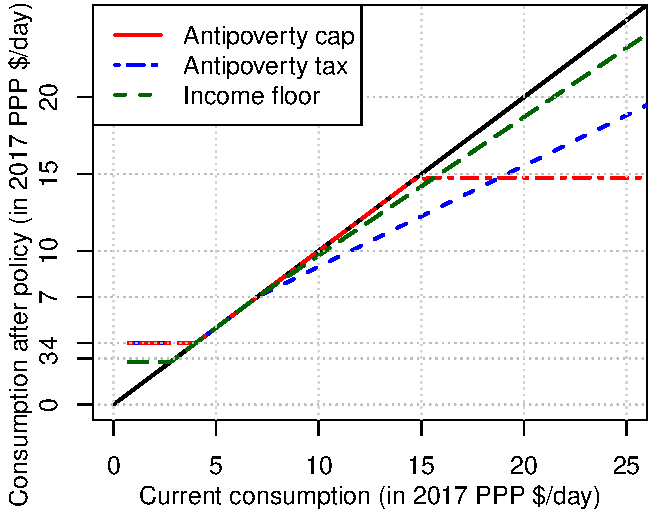
\includegraphics[width=\textwidth]{../figures/Kenya_policies.pdf}
  \end{subfigure} \;
  \begin{subfigure}{.5\textwidth}
    \caption[]{Anti-\textit{\$4-poverty} cap: \$14.8/day.}\label{fig:kenya_cap}
    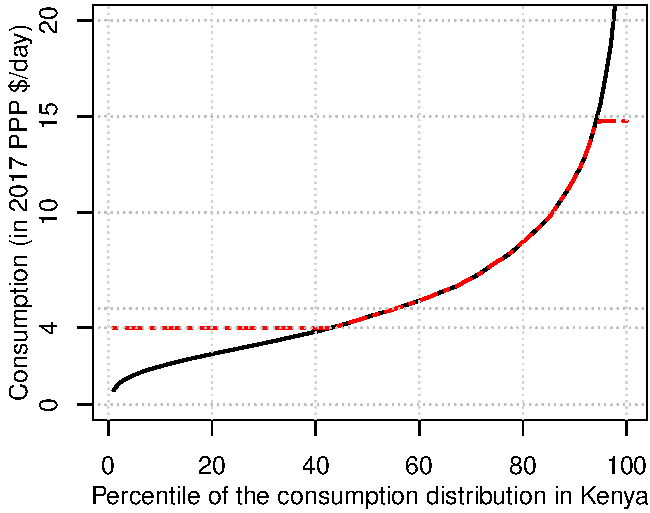
\includegraphics[width=\textwidth]{../figures/Kenya_cap.pdf}
  \end{subfigure}
  \\ \quad \\
  \begin{subfigure}{.5\textwidth}
    \caption[]{Anti-\textit{\$4-poverty} tax (above \$7/day): 34\%.}\label{fig:kenya_tax}
    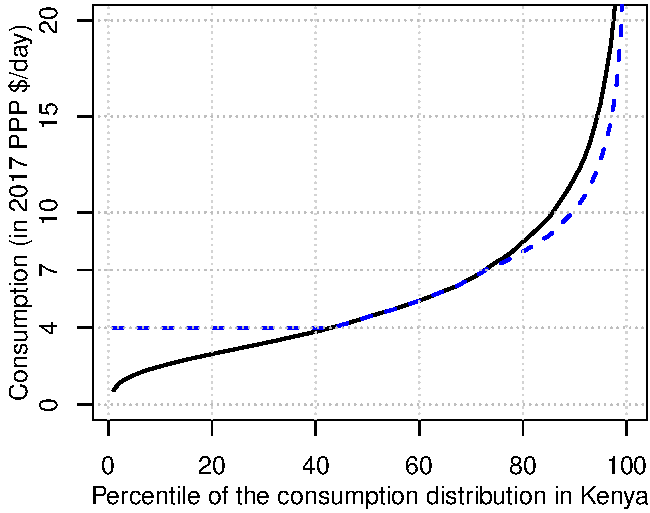
\includegraphics[width=\textwidth]{../figures/Kenya_tax.pdf}
  \end{subfigure} \;
  \begin{subfigure}{.5\textwidth}
    \caption[]{Income floor (funded by a 10\% tax above \$7/day): \$2.8/day.}\label{fig:kenya_floor}
    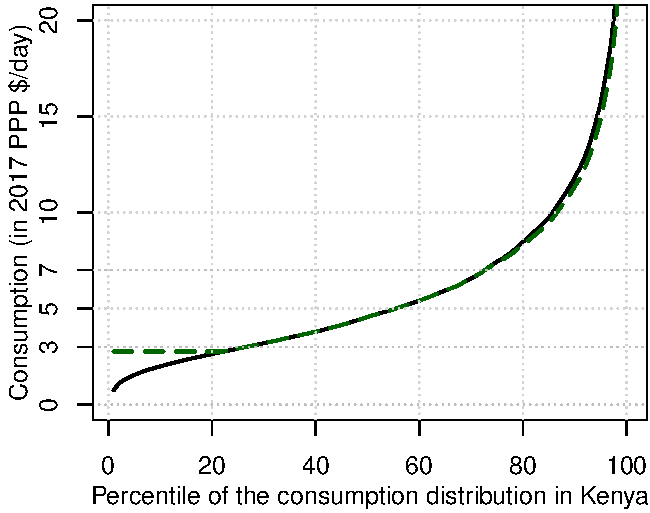
\includegraphics[width=\textwidth]{../figures/Kenya_floor.pdf}
  \end{subfigure}
\end{figure}  

These policies are idealized. The estimate of revenue they generate should be seen as an upper bound of what could be achieved if they were implemented in practice. 
First, I ignore any costs associated with raising a tax or transferring money, as if the lowest-income countries already had sufficient administrative resources. Second, any tax (and a fortiori a 100\% tax) reduces economic activity (real or declared). In this exercise, I abstract from tax distorsions and assume that the policies would not affect the taxable base.%

If it were possible to expropriate top income individuals 
without reducing their economic activity, capping top incomes to finance an income floor would eliminate poverty at the lowest welfare cost. 
However, to protect private property and diminish the deterring effect on economic activity, governments would rather tax at a lower rate (than 100\%) and on a broader base (starting at a threshold deemed reasonable). 
Therefore, the antipoverty cap, the antipoverty tax, and the income floor can be thought as rough but revealing approximations of the capacity to mobilize domestic resources. The paper's estimates should not be viewed as causal outcomes of the effects of the idealized policies simulated.

In low-income countries, we measure household consumption rather than income, meaning that we do not capture investment nor government spending. In other words, our idealized policies would leave productive investment and public services unaffected, an appropriate treatment given that these channels already contribute to growth and poverty reduction.%

Unless otherwise stated, I use the scenario of balanced growth at a rate of 3\%. I choose this rate as a baseline as it is an upper bound of growth rates recently experienced in the lowest-income countries. Indeed, among the 8 countries with an average consumption below 3\$/day, growth was on average negative over 2014--2019 (or 2014--2022), and the highest growing country (Central African Republic) grew at a rate of 2.4\% per year. %

\subsection{Antipoverty caps\label{subsec:cap}}

\begin{figure}[!b]
  \caption[Anti-\textit{extreme-poverty} cap in 2030 after 3\% growth.]{Income cap eradicating extreme poverty (in \$/day). In this idealized policy, all income above the cap is transferred to the extreme poor and lift them at \$2.15/day, assuming away distorsions, and after a yearly growth of 3\% over 2022--2030. %
  }\label{fig:antipoverty_cap}
  \makebox[\textwidth][c]{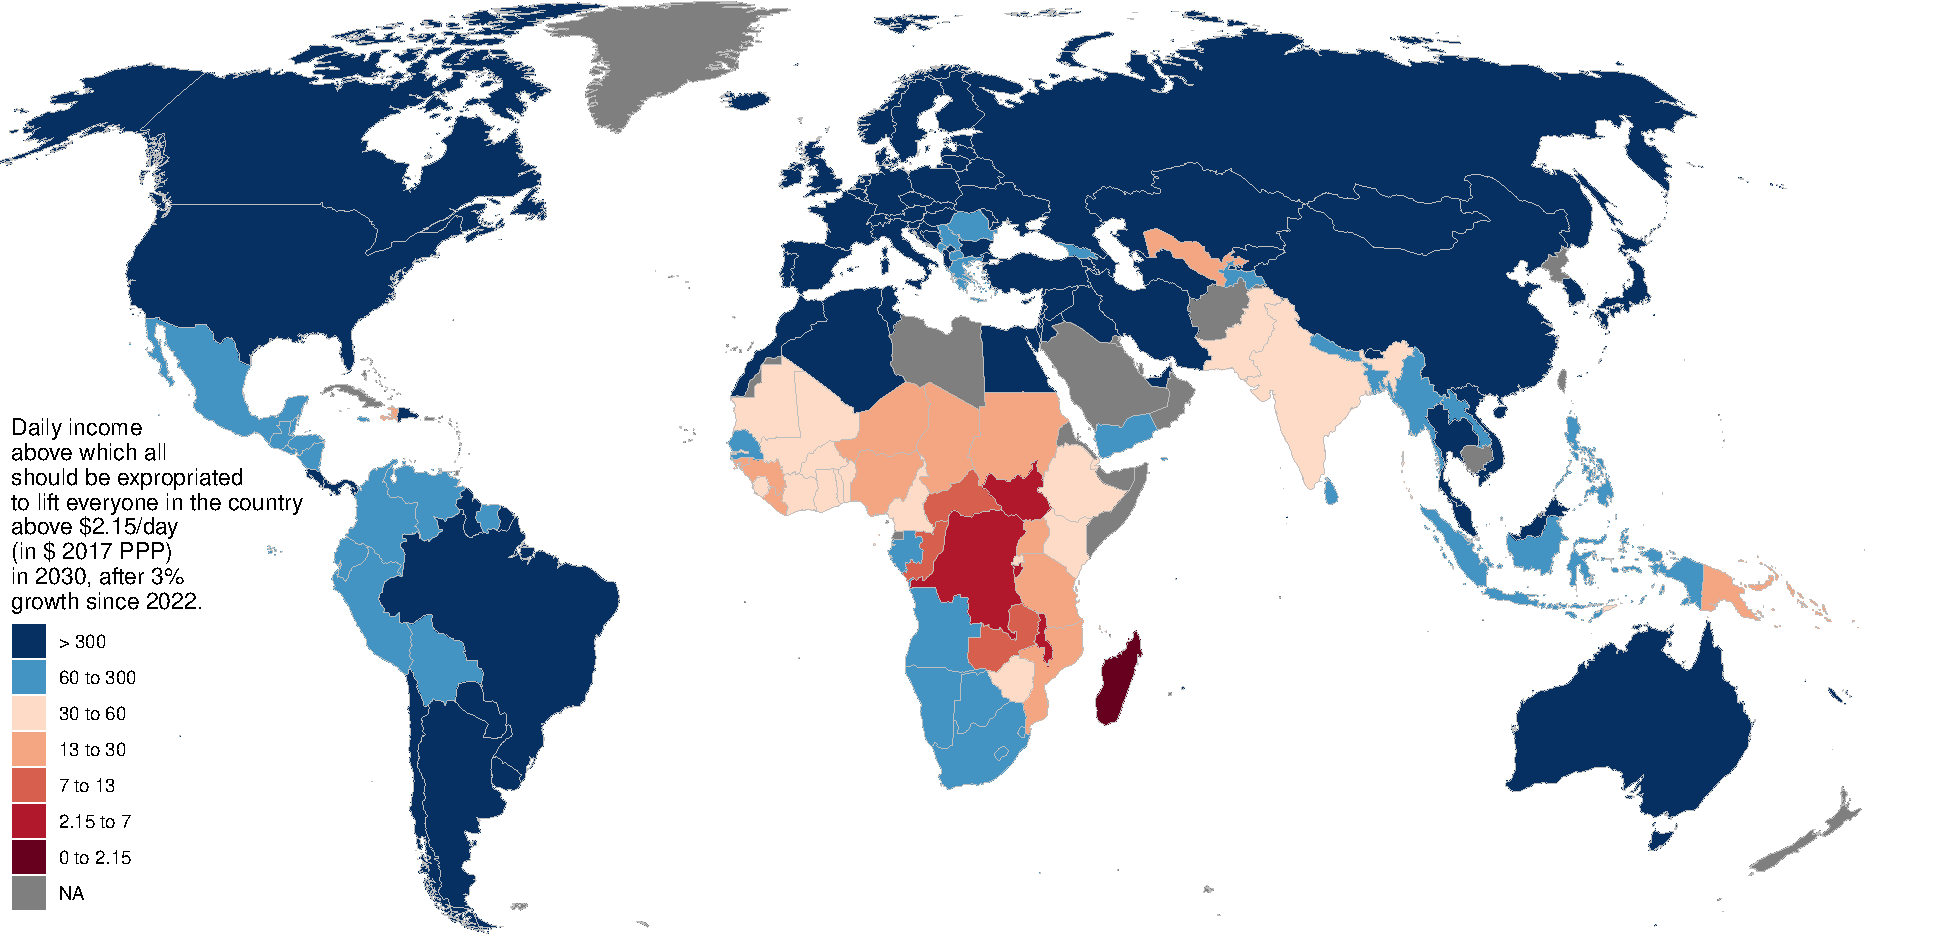
\includegraphics[width=\textwidth]
  {../figures/antipoverty_2_cap_average.pdf}}
\end{figure} 

I estimate the income cap that each country should impose to fill the extreme poverty gap with the expropriated income, i.e. all income above the cap (Figure \ref{fig:antipoverty_cap}). 
In some low-income countries, even capping incomes at \$7/day would not suffice to raise revenues equal to the extreme poverty gap, despite a steady growth of 3\% per year between 2022 and 2030. 
In a very optimistic scenario of 7\% growth, the anti-\textit{extreme-poverty} cap would be \$14/day in the D.R.C. Also, note that there is no indication that the resources of this country are underestimated, as the aggregate consumption from household surveys is greater than HFCE %
from national accounts for the D.R.C. 
Besides, the D.R.C. is not the poorest country. 
In Madagascar, the average consumption would fall short of \$2.15/day in the baseline scenario, at \$2.02/day. This means that even with extreme redistribution, Madagascar does not have the domestic resources needed to eliminate extreme poverty by 2030. 
To give one last example of the shortfall of resources in the lowest-income countries, the anti-\textit{extreme-poverty} cap for Burundi in the scenario of 7\% growth would need to be as low as 8.60\$/day. 

\paragraph{Accounting for country-specific prices of subsistence goods.}
In most of the paper, I focus on the definition of extreme poverty employed in the first SDG. However, the \$2.15 cut-off has been criticized for inaccurately measuring poverty \citep{woodward_redefining_2010,deaton_price_2010,deaton_purchasing_2011}. %
First, this poverty line %
is barely sufficient to satisfy one's caloric requirements and is too low to procure a healthy diet or non-food necessities. 
Second, the PPP adjustments applied to PIP data before computing the poverty rates are based on prices of an average consumption basket rather than on prices of subsistence goods \citep{sullivan_capitalist_2023}. Therefore, the cost of a subsistence diet varies across countries. For instance, \cite{moatsos_global_2016} computes that it is \$1.44 in Malawi vs. \$4.10 in Kenya (in 2011 PPP \$). Buidling on earlier work by \cite{allen_absolute_2017} that addresses these issues, \cite{moatsos_global_2016} computes a country-specific poverty line. This basic consumption (or \textit{BCS}) poverty line corresponds to the local price of the cheapest diet that meets caloric and protein requirements, completed with a ration of fat, sugar, and basic non-food requirements (see also \citealp{moatsos_global_2021}). This alternative measure, equal to \$4.35/day in median, indicates that poverty %
is more prevalent than the official poverty line suggests. Despite missing data in many countries (including India and the D.R.C.), 14 countries have an average consumption level below this basic consumption poverty line in 2030 in the 3\% growth scenario. These countries (which include e.g. Nigeria) do not have sufficient resources to lift their population above the BCS poverty line even after an extreme domestic redistribution that would equalize all incomes. 

\paragraph{Comparing results to previous estimates.}
BCL found that 62 countries could not eradicate severe poverty (defined as \$$_\text{2005}$2/day) with an antipoverty cap at \$$_\text{2005}$13/day, while 27 could not even do so with a cap at \$$_\text{2005}$2/day. 
Their findings cannot be exactly reproduced with the revised PIP data, as the switch from 2005 to 2017 PPPs has altered not only the level but also the distribution of incomes (for the same reason, the results of BCL and \cite{ravallion_poorer_2010} cannot be compared). 
When I replicate the computations of BCL (with their survey years but after scaling the original cut-offs into 2017 PPPs by a factor $2.15/1.25 = 1.72$), I find that 53 (resp. 30) 
countries could not eradicate severe poverty with a cap at \$22.36/day (resp. \$3.44/day). 
Looking ahead, in our baseline scenario with 3\% growth, I find that in 2030, 34 (resp. 6) 
countries will not be able to eradicate severe poverty with a cap at \$22.36/day (resp. \$3.44/day). In other words, growth significantly reduces poverty and increases the capacity of low-income countries to eradicate poverty.

\subsection{Antipoverty taxes\label{subsec:tax}}

\begin{figure}[b!]
  \caption[Anti-\textit{extreme-poverty} tax above \$6.85/day in 2030 after 3\% growth.]{Linear tax rate above \$6.85/day eradicating extreme poverty (in \%). In this idealized policy, all tax revenue is transferred to the extreme poor and lift them at \$2.15/day, assuming away distorsions, and after a yearly growth of 3\% over 2022--2030. 
  }\label{fig:antipoverty_tax_7}
  \makebox[\textwidth][c]{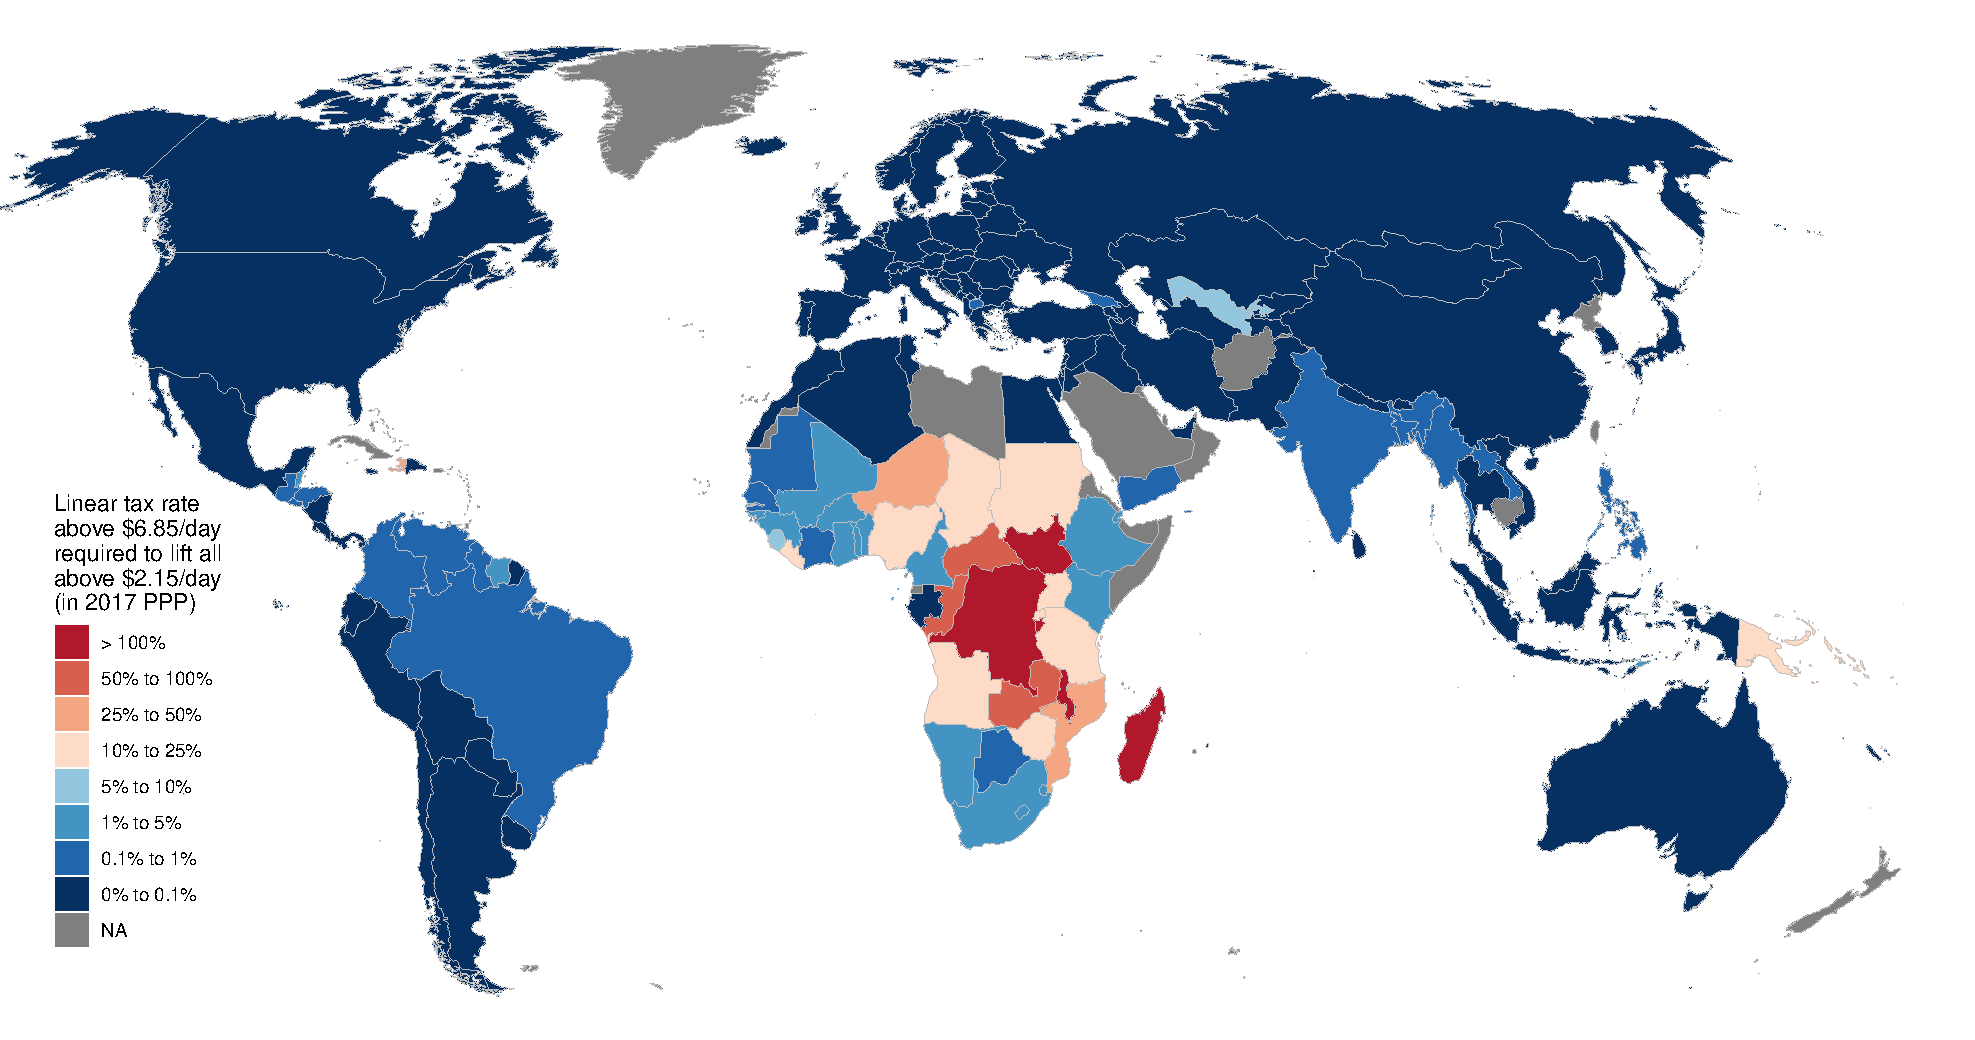
\includegraphics[width=\textwidth]
  {../figures/antipoverty_2_tax_7_average.pdf}}
\end{figure}

Figure \ref{fig:antipoverty_tax_7} presents the tax rate above \$6.85/day required to generate enough revenues to close the domestic extreme poverty gap, in the baseline scenario of 3\% growth. %
The cut-off of \$6.85/day is defined by the World Bank as the median national poverty line of upper middle-income countries. It corresponds to an ``acute'' poverty line which can be understood as the consumption level that can sustain a minimally decent life \citep{hickel_is_2019,kikstra_decent_2021}. In contrast, the extreme poverty line of \$2.15/day corresponds to the consumption per capita below which one is undernourished \citep{allen_absolute_2017}. 

Consistently with the previous findings, taxing income at a 100\% rate above \$6.85/day would not generate enough revenues to eliminate extreme poverty in the five poorest countries. In Nigeria, closing the extreme poverty gap would require taxing the ``non-acutely-poor'' at a marginal rate of 20\%. 
On average over Sub-Saharan Africa, the anti-\textit{extreme-poverty} tax would be 46\%, and 70\% in low-income countries (defined by the World Bank as countries with a GNI per capita below \$1,135 per year). Yet, imposing such a large tax burden on any income above just \$6.85/day seems unrealistic. 

\begin{figure}[h!]
  \caption[Anti-\textit{extreme-poverty} tax above \$18.15/day in 2030 after 3\% growth.]{Linear tax rate above \$18.15/day eradicating extreme poverty (in \%). In this idealized policy, all tax revenue is transferred to the extreme poor and lift them at \$2.15/day, assuming away distorsions, and after a yearly growth of 7\% over 2022--2030.
  }\label{fig:antipoverty_tax_18}
  \makebox[\textwidth][c]{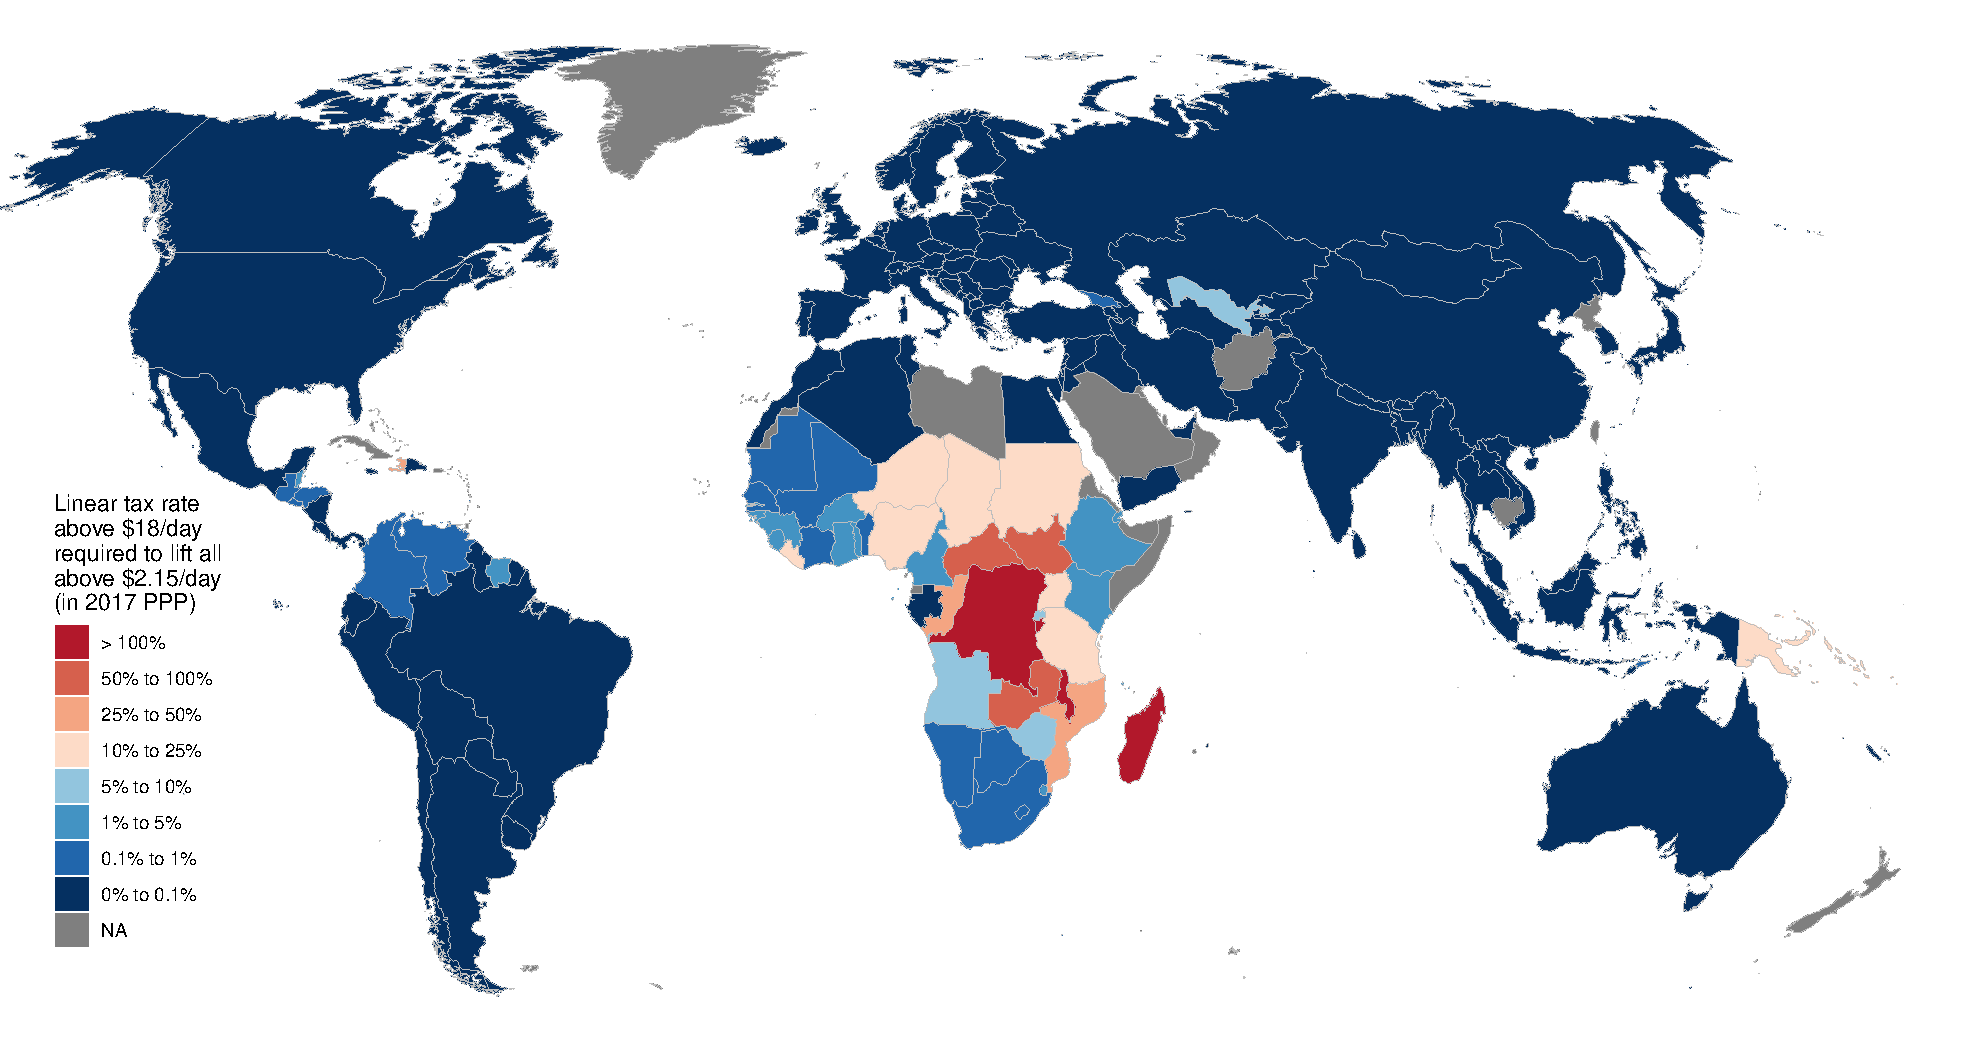
\includegraphics[width=\textwidth]
  {../figures/antipoverty_2_tax_18_very_optimistic.pdf}}
\end{figure}

Figure \ref{fig:antipoverty_tax_18} presents the anti-\textit{extreme-poverty} tax on incomes above \$18.15/day, in a very optimistic scenario of 7\% growth. The threshold of \$18.15/day per person corresponds to the U.S. federal poverty line for a family of four and represents a more realistic threshold above which taxes could be increased in the Global South. The anti-\textit{extreme-poverty} tax rates on the ``non-poor'' %
in this 7\% growth scenario are comparable to the rates on the non-acutely-poor in the baseline scenario. In India, the required tax rate would be 10\% %
in the scenario with 7\% growth until 2030, 36\% with 5.5\% growth (the country's 2014--2019 trend), and unachievable (at 156\%) with 3\% growth. %
With sustained growth, the contribution required of the Indian non-poor seems large but possible. %
Therefore, India seems able to eliminate extreme poverty by 2030 with its domestic resources. The same thing cannot be said of Sub-Saharan Africa. %
\subsection{Income floor as a measure of credible potential for redistribution\label{subsec:floor}}

A final way of approaching the issue is to set a tax schedule, compute how much revenue it would generate in each country, and estimate the income floor that these revenues could finance (by topping up the incomes of the poorest to the income floor). Note that the value of the income floor depends on the whole income distribution: the top of the distribution determines the revenues that can be generated; and the bottom dictates the cost of raising low incomes up to a given floor. As I have already explored extreme redistributive policies, I analyse here a more reasonable tax schedule. Namely, I consider a 10\% marginal tax rate on income above \$6.85/day. Although the tax base I choose may be too wide (affecting people on the verge of acute poverty) %
and the tax rate too low for top incomes, 
this simple tax schedule seems to correctly reflect the fiscal capacity of governments. Indeed, this tax schedule is conservatively inspired by \cite{ravallion_poorer_2010}, who uses a rate of 10\% but a higher threshold (corresponding to \$18/day) to assess whether a country has a high or low capacity to eradicate poverty. 

Figure \ref{fig:demogrant_7__10} presents the income floor that can funded in 2030 with our simple tax in a 3\% growth scenario. 23 countries are unable to eradicate extreme poverty with this tax. This figure is close to the count of low-income countries, at 27, but only 13 countries fall into both categories.
For example, while Ethiopia (a low-income country) can finance an income floor of \$3.08/day, Nigeria (classified as a lower-middle-income country) can only finance a floor of \$1.83/day. 

\begin{figure}[t!]
  \caption[Income floor of 10\% tax above \$6.85/day in 2030 after 3\% growth.]{Income floor that can be funded with a 10\% marginal tax on income above \$6.85/day (in 2017 PPP \$/day). In this idealized policy, all tax revenue is transferred to the poorest and lift them at the income floor, assuming away distorsions, and after a yearly growth of 3\% over 2022--2030. 
  }\label{fig:demogrant_7__10}
  \makebox[\textwidth][c]{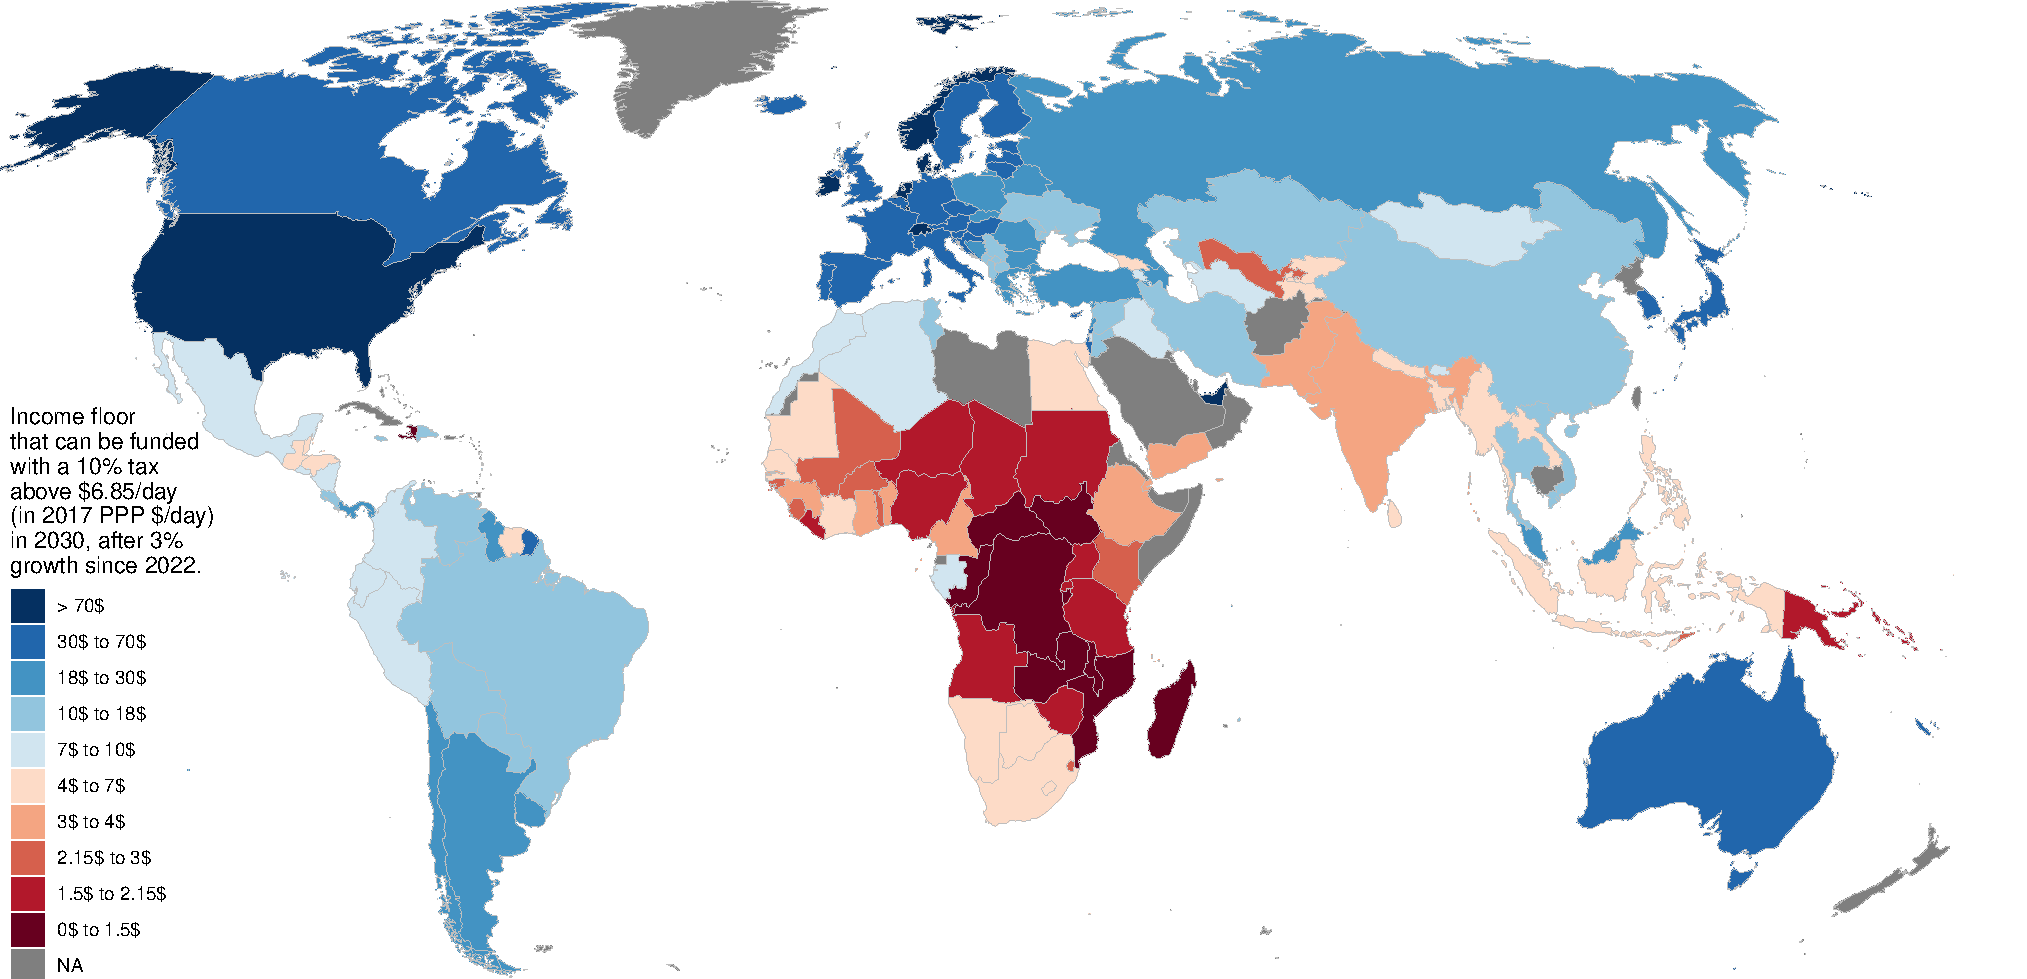
\includegraphics[width=\textwidth]
  {../figures/floor_7__10.pdf}}
\end{figure}

Even in a scenario with 7\% growth from 2023 onwards, 10 countries have an income floor below \$2.15 in 2030. Note that the picture does not significantly change when adjusting top incomes so that aggregate consumption matches national accounts: %
8 countries are still unable to close the extreme poverty gap despite very optimistic growth in this robustness check. In contrast, if the 7\% growth had started in 2016 (as the SDGs were set up), the 10\% tax would have been sufficient to eliminate extreme poverty in all countries except in Madagascar, where a tax of 23\% would have been required.

\paragraph{Two paths to alleviate poverty.}
At least two of the SDGs spell out how the elimination of extreme poverty could be funded. %
First, the target 8.1 aims for ``at least 7 per cent gross domestic product growth per annum in the least developed countries''. As we have seen, a sustained high growth since 2016 would have permitted the least developed countries to eliminate extreme poverty through the mobilization of their domestic resources. However, high growth has never materialized in these countries. 
Second, the target 17.2 calls for ``Developed countries to implement fully their official development assistance commitments, including the commitment by many developed countries to achieve the target of 0.7 per cent of ODA/GNI to developing countries and 0.15 to 0.20 per cent of ODA/GNI to least developed countries'' (LDCs). Foreign aid falls short of both the overall target (at 0.37\% of developed countries' GNI) and the LDCs' target (at 0.06\%). While just four countries are meeting their commitments (Luxembourg, Sweden, Norway, and Germany), the U.S. only allocates 0.23\% of its GNI to foreign aid \citep{oecd_oda_2023}. The global extreme poverty gap (predicted at 0.17\% of global real GDP in 2030) is a bit lower than the shortfall of foreign aid relative to the target (0.2\% of global nominal GDP), suggesting that extreme poverty could be significantly reduced if developed countries respected their commitment. %
However, to meet the broader SDGs and ``end poverty in all its forms'', the 0.7\% target would not suffice and international solidarity should be significantly strenghtened. %

\subsection{The potential of global redistribution\label{subsec:global}} %

In this section, we highlight the potential of globally redistributive policies to close the global poverty gap in 2030 in the baseline scenario of 3\% growth. The policies described are idealized and should be understood as proxies for any action of international solidarity or system change that would bring about an equivalent transfer of resources. %

If applied to the global level, the tax of the previous section would bring the global Gini from .62 down to .51 and finance an income floor at \$8.6/day, thereby closing the \$6.85/day poverty gap. By comparison, applied at the national level, it would only bring the global Gini down to .59 and reduce the poverty gap from 4.5\% to 3.7\% of global income. 

To close the \textit{extreme} poverty gap, a 1.2\% marginal tax %
above 100\$/day (i.e. \$36,500/year) would suffice. %
Such a tax would result in 0.15\% of global income being transferred from the rich to the extreme poor, and almost exclusively transferred from rich countries to poor countries. 
With contributions of up to 0.4\% of a country's income (in the U.S.), aggregate consumption would increase by more than 10\% in 9 countries. 

In reality, the global tax rates required to eradicate poverty may well be lower than just indicated, because our calculations used the raw PIP data instead of converting them to nominal terms and rescaling them to national accounts. Once I rescale the data to national accounts (which are more accurate in high-income countries), %
a mild 0.3\% marginal tax above \$100/day suffices to close the extreme poverty gap. Raising that rate to 10\% would collect 3.4\% of the world income, enough to finance a global income floor of \$7/day and end absolute poverty ``in all its forms'' (extreme and acute). %
These rates are expressed on top of the current tax system and apply to post-tax income. For example, the last tax schedule would leave unaffected the 95\% of the world's population whose per capita after-tax income is less than \$36,500/year, and would reduce the after-tax income of those at \$73,000/year by 5\%. 
Although internationally redistributive taxes have yet to take off, the proposal of a global wealth tax is gaining momentum \citep{piketty_brief_2022}. A 2\% tax on individual net wealth above \$1 billion would raise \$214 billion a year, slightly more than the global extreme poverty gap \citep{alstadsaeter_global_2024}. Moreover, a global tax on the wealthiest 1\% can raise enough revenues to close the global acute poverty gap and lift everyone above \$6.85/day. For example, the \href{https://wid.world/world-wealth-tax-simulator}{WID wealth tax simulator} shows that a tax consisting of a 4\% marginal rate above \$1 million and 10\% above \$100 million would raise 4.4\% of the global GDP. More generally, a global tax on millionaires designed to be revenue-maximing in the long-run has the potential to finance the eradication of acute poverty. 

While global solidarity has the potential to eradicate poverty, one may wonder whether it is politically and technically feasible. 
Regarding political acceptability, while government support seems currently unlikely, \cite{fabre_international_2023} show overwhelming public support for a global tax on millionaires that would finance low-income countries, reaching 69\% support in the U.S. and 84\% in Europe. %
As for implementation, government programs offer a proven path to poverty reduction through the deployment of public services, social protection, and infrastructures. 
Admittedly, our idealized policies entail direct cash transfers to the poorest households. Such transfers are viewed as a promising way to alleviate poverty \citep{haushofer_short-term_2016,egger_general_2022}, but could be challenging to implement. In this regard, progress in payment infrastructures has been encouraging. In particular, the World Bank's \textit{Identification for Development} program finances identification systems in 57 of the world's poorest countries \citep{world_bank_state_2017,world_bank_benin_2020,world_bank_identification_2022}, with the aim of ``providing legal identity for all'' in line with SDG n\textdegree{}16.9. This identification makes it possible to offer numerous services, including cash transfers. In India, the Aadhaar system has provided a unique biometric identifier for 99\% of the adult population in just 8 years. Aadhaar is linked to bank accounts and already used to distribute social benefits \citep{muralidharan_identity_2023}. In less than two weeks, Togo has set up a mobile money transfer for one million people to compensate for the loss of income suffered by informal workers in confined areas during the COVID pandemic \citep{ipa_togos_2021}. Finally, affordable satellite internet and solar panels are making mobile payments accessible in remote areas. %

In a nutshell, whereas poverty alleviation cannot be achieved rapidly without international solidarity, it can be financed by reasonable contributions from the global top 1\%.

\section{Discussion\label{sec:conclusion}} 

To paraphrase the \cite{un_sustainable_2022}, ``as things stand, the world is not on track to end poverty by 2030.'' I have shown that the only prospect for low-income countries to eliminate extreme poverty on their own is the combination of strong growth, ambitious social programs and domestic redistribution, and time. 
With record growth and profound government committment, China has officially eradicated extreme poverty in 2021. The D.R.C. is poorer today than China was in 1990, %
so even if the D.R.C. replicates the Chinese miracle, which is not easy given its institutional capacity, the D.R.C. will not be able to eradicate extreme poverty on its own before 2055. %
In contrast, international solidarity might be able to end poverty more quickly and at a much lower welfare cost. In this paper, I have illustrated the magnitude of the required transfer of resources with idealized international taxes, but in reality this could take other forms such as a systemic change in the rules or structures of the world economy. 
To be fair, this paper only presents the orders of magnitude of global inequality. %
In practice, structural factors that sustain poverty (like wars or corruption) %
can also hamper the effectiveness of international action. %

Finally, a number of limitations prevent the paper from providing definitive estimates of domestic capacities to eradicate poverty. First, while PIP arguably provides the most appropriate data to measure absolute poverty, it does not adequately capture investment, government spending, and top incomes. To better capture in-kind consumption of public services, \cite{fisher-post_government_2023} offer a promising database, though poverty lines would need to be adjusted accordingly. Second, estimates could be improved when PIP releases a data update, with more recent surveys and prices expressed in 2023 PPP~\$. Third, the poverty gap may not be the most accurate measure of the resources needed to eradicate poverty. Instead, it may be more relevant to consider non-economic factors like education and healthcare access, or government programs like social assistance, and assess their cost.

  \begin{small} %

% \section*{\normalsize Data and code availability}

% All data and code of as well as figures of the paper are available on \href{https://github.com/bixiou/domestic_poverty_eradication}{github.com/bixiou/domestic\_poverty\_eradication}. Many more figures (with varying poverty lines, taxation thresholds, growth scenarios, etc.) are available on the repository. %
% Also, any custom figure can be easily produced using this code. The article also comes with a Figshare DOI: \href{https://figshare.com/articles/dataset/dx_doi_org_10_6084_m9_figshare_6025748/6025748}{10.6084/m9.figshare.28229477}.

\end{small}  %

\theendnotes

\bibliography{poverty}

\begin{itemize}
\item[JEL codes] D63, I32, P16.
\item[Keywords]  Poverty gap, Sustainable Development Goals, Domestic resource mobilization, Redistribution, Fiscal capacity, Extreme poverty.
\end{itemize}

\listoftables
\listoffigures

\appendix %
\renewcommand{\thetable}{A\arabic{table}}
\renewcommand{\thefigure}{A\arabic{figure}}
\setcounter{figure}{0}
\setcounter{table}{0}

\end{document}
